\begin{center}
\underline{\Large{T.P.N°2: Losas}}
\end{center}

\begin{enumerate}
\item a) Dada la planta de arquitectura de la Figura 1, definir la planta estructural, señalando la posición de columnas, vigas y losas. Representar el resultado a escala. b) Para las losas correspondientes al balcón, la sala de computación, el archivo y la sala de reunión de la Figura 1, efectuar el análisis de cargas según el esquema del inciso a) (considerar las cargas generadas por las paredes), determinar el espesor adecuado según los requerimientos de rigidez y dimensionarlas. Desarrollar el cálculo según CIRSOC 201-05 y según CIRSOC 201-82, comparando los resultados. c) Dibujar el plano estructural adoptado y el plano de armado de las losas solicitadas. Considerar las losas pertenecientes a núcleos húmedos como descendidas.\\

\begin{figure}[H]
\begin{center}
     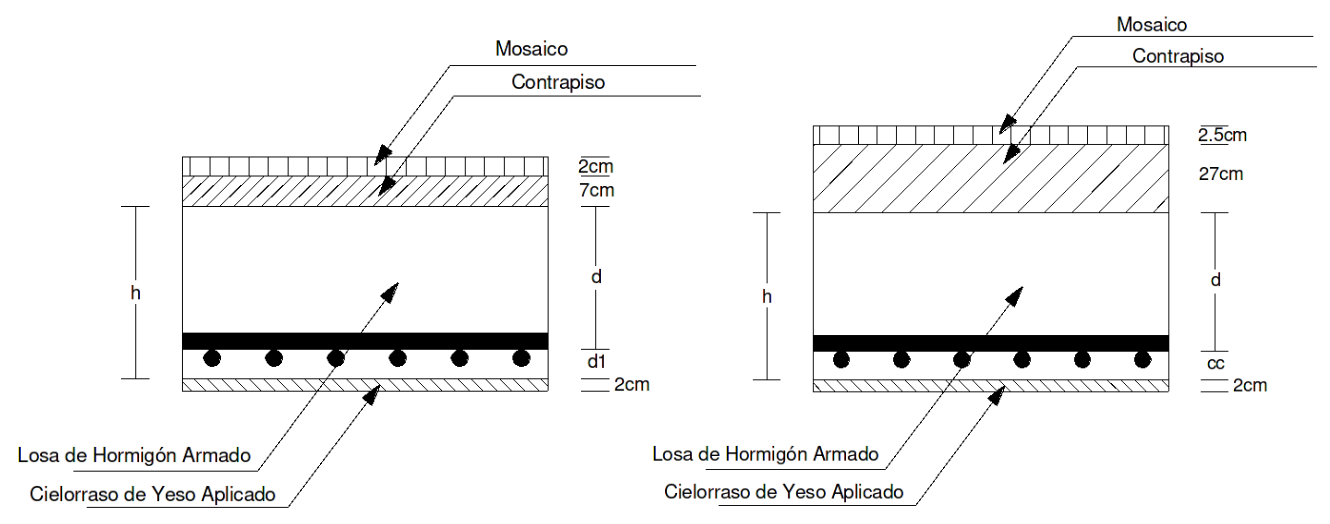
\includegraphics[scale = 0.9]{chapters/chapter_1/images/paquete_piso.png}
\end{center}
\end{figure}

\item Para la planta estructural de la azotea de un edificio de la Figura 2, calcular y dibujar el plano de armado de la losa Nº 302. Realizar el cálculo según Reglamento CIRSOC 201-05.

\item a) Indicar el esquema de sustentación para el cálculo del sistema de losas de la Figura 3. b) Esquematizar el diagrama de momentos y su armado, señalando las armaduras que resultan principales y secundarias, superiores e inferiores. c) En la losa 304 de la Figura 3 debe ubicarse un orificio de 1 m por 1 m para el paso de un pequeño montacargas. Efectuar el detalle del armado del orificio de la losa e indicar el procedimiento que llevaría a cabo para calcular la armadura de refuerzo.

\begin{figure}[H]
\begin{center}
     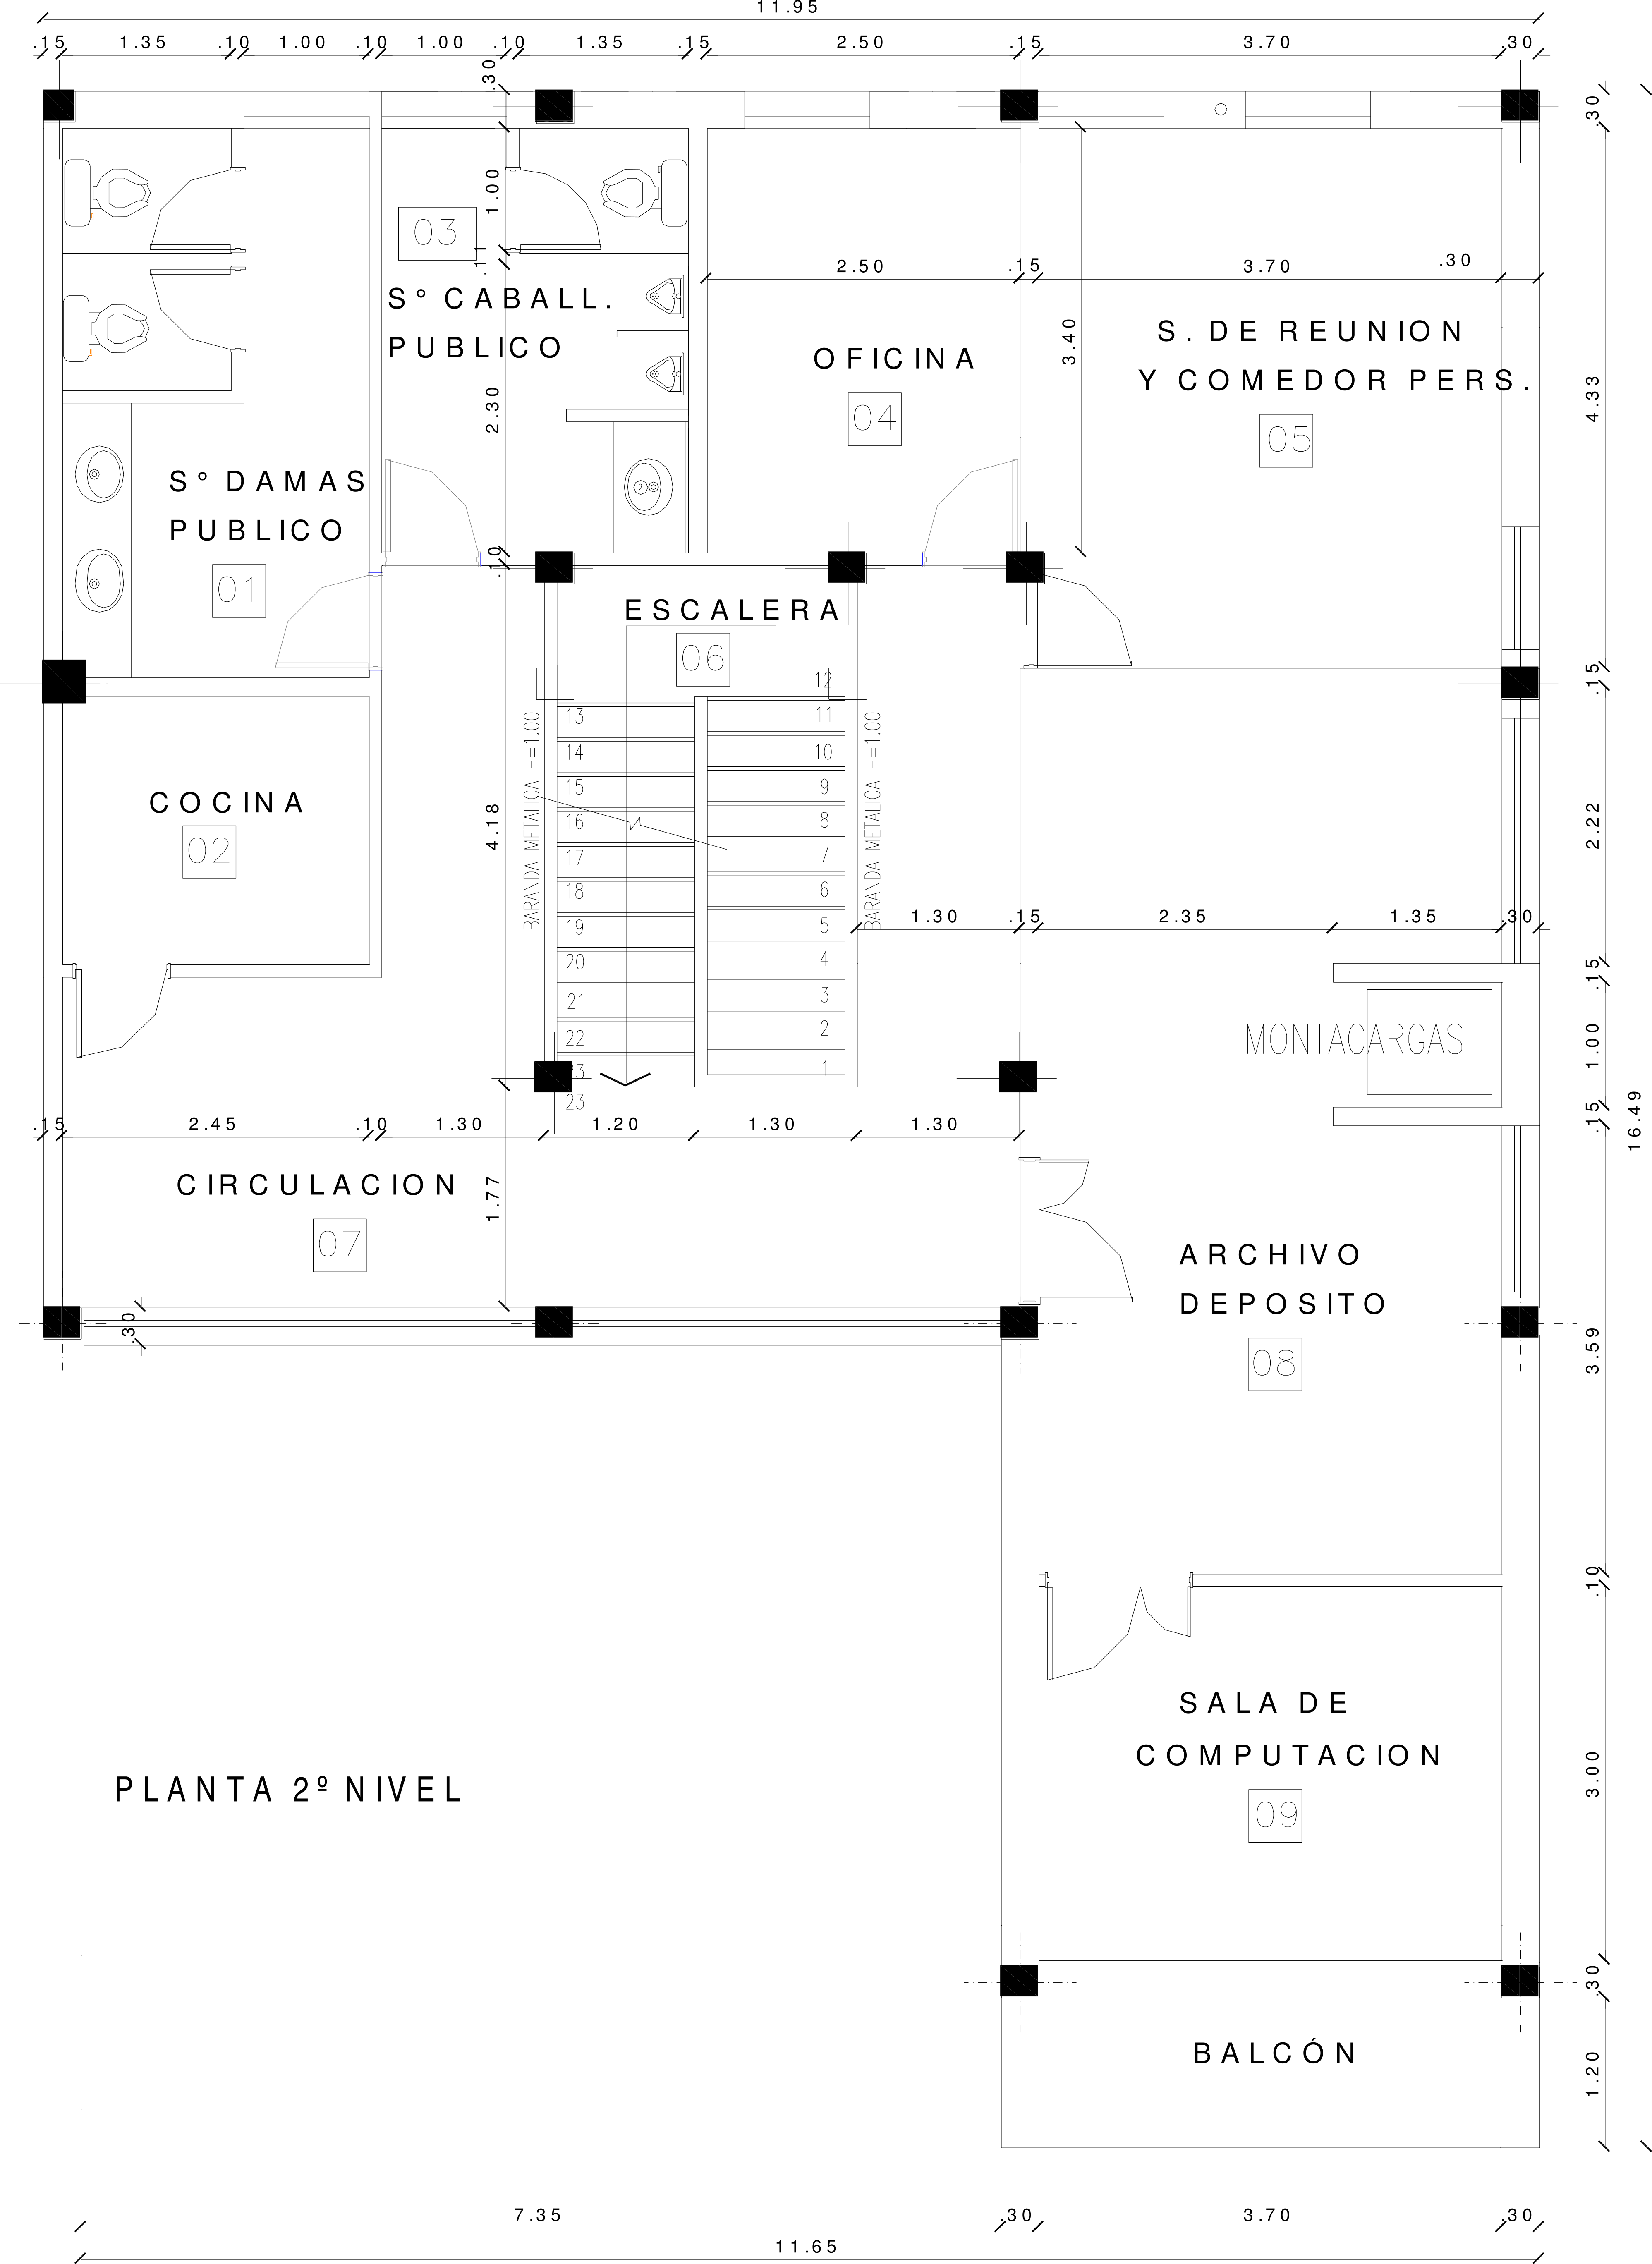
\includegraphics[scale = 0.9]{chapters/chapter_1/images/figura1.png}
\end{center}
\caption{Planta de arquitectura para el ejercicio 1}
\end{figure}

\begin{figure}[H]
\begin{center}
     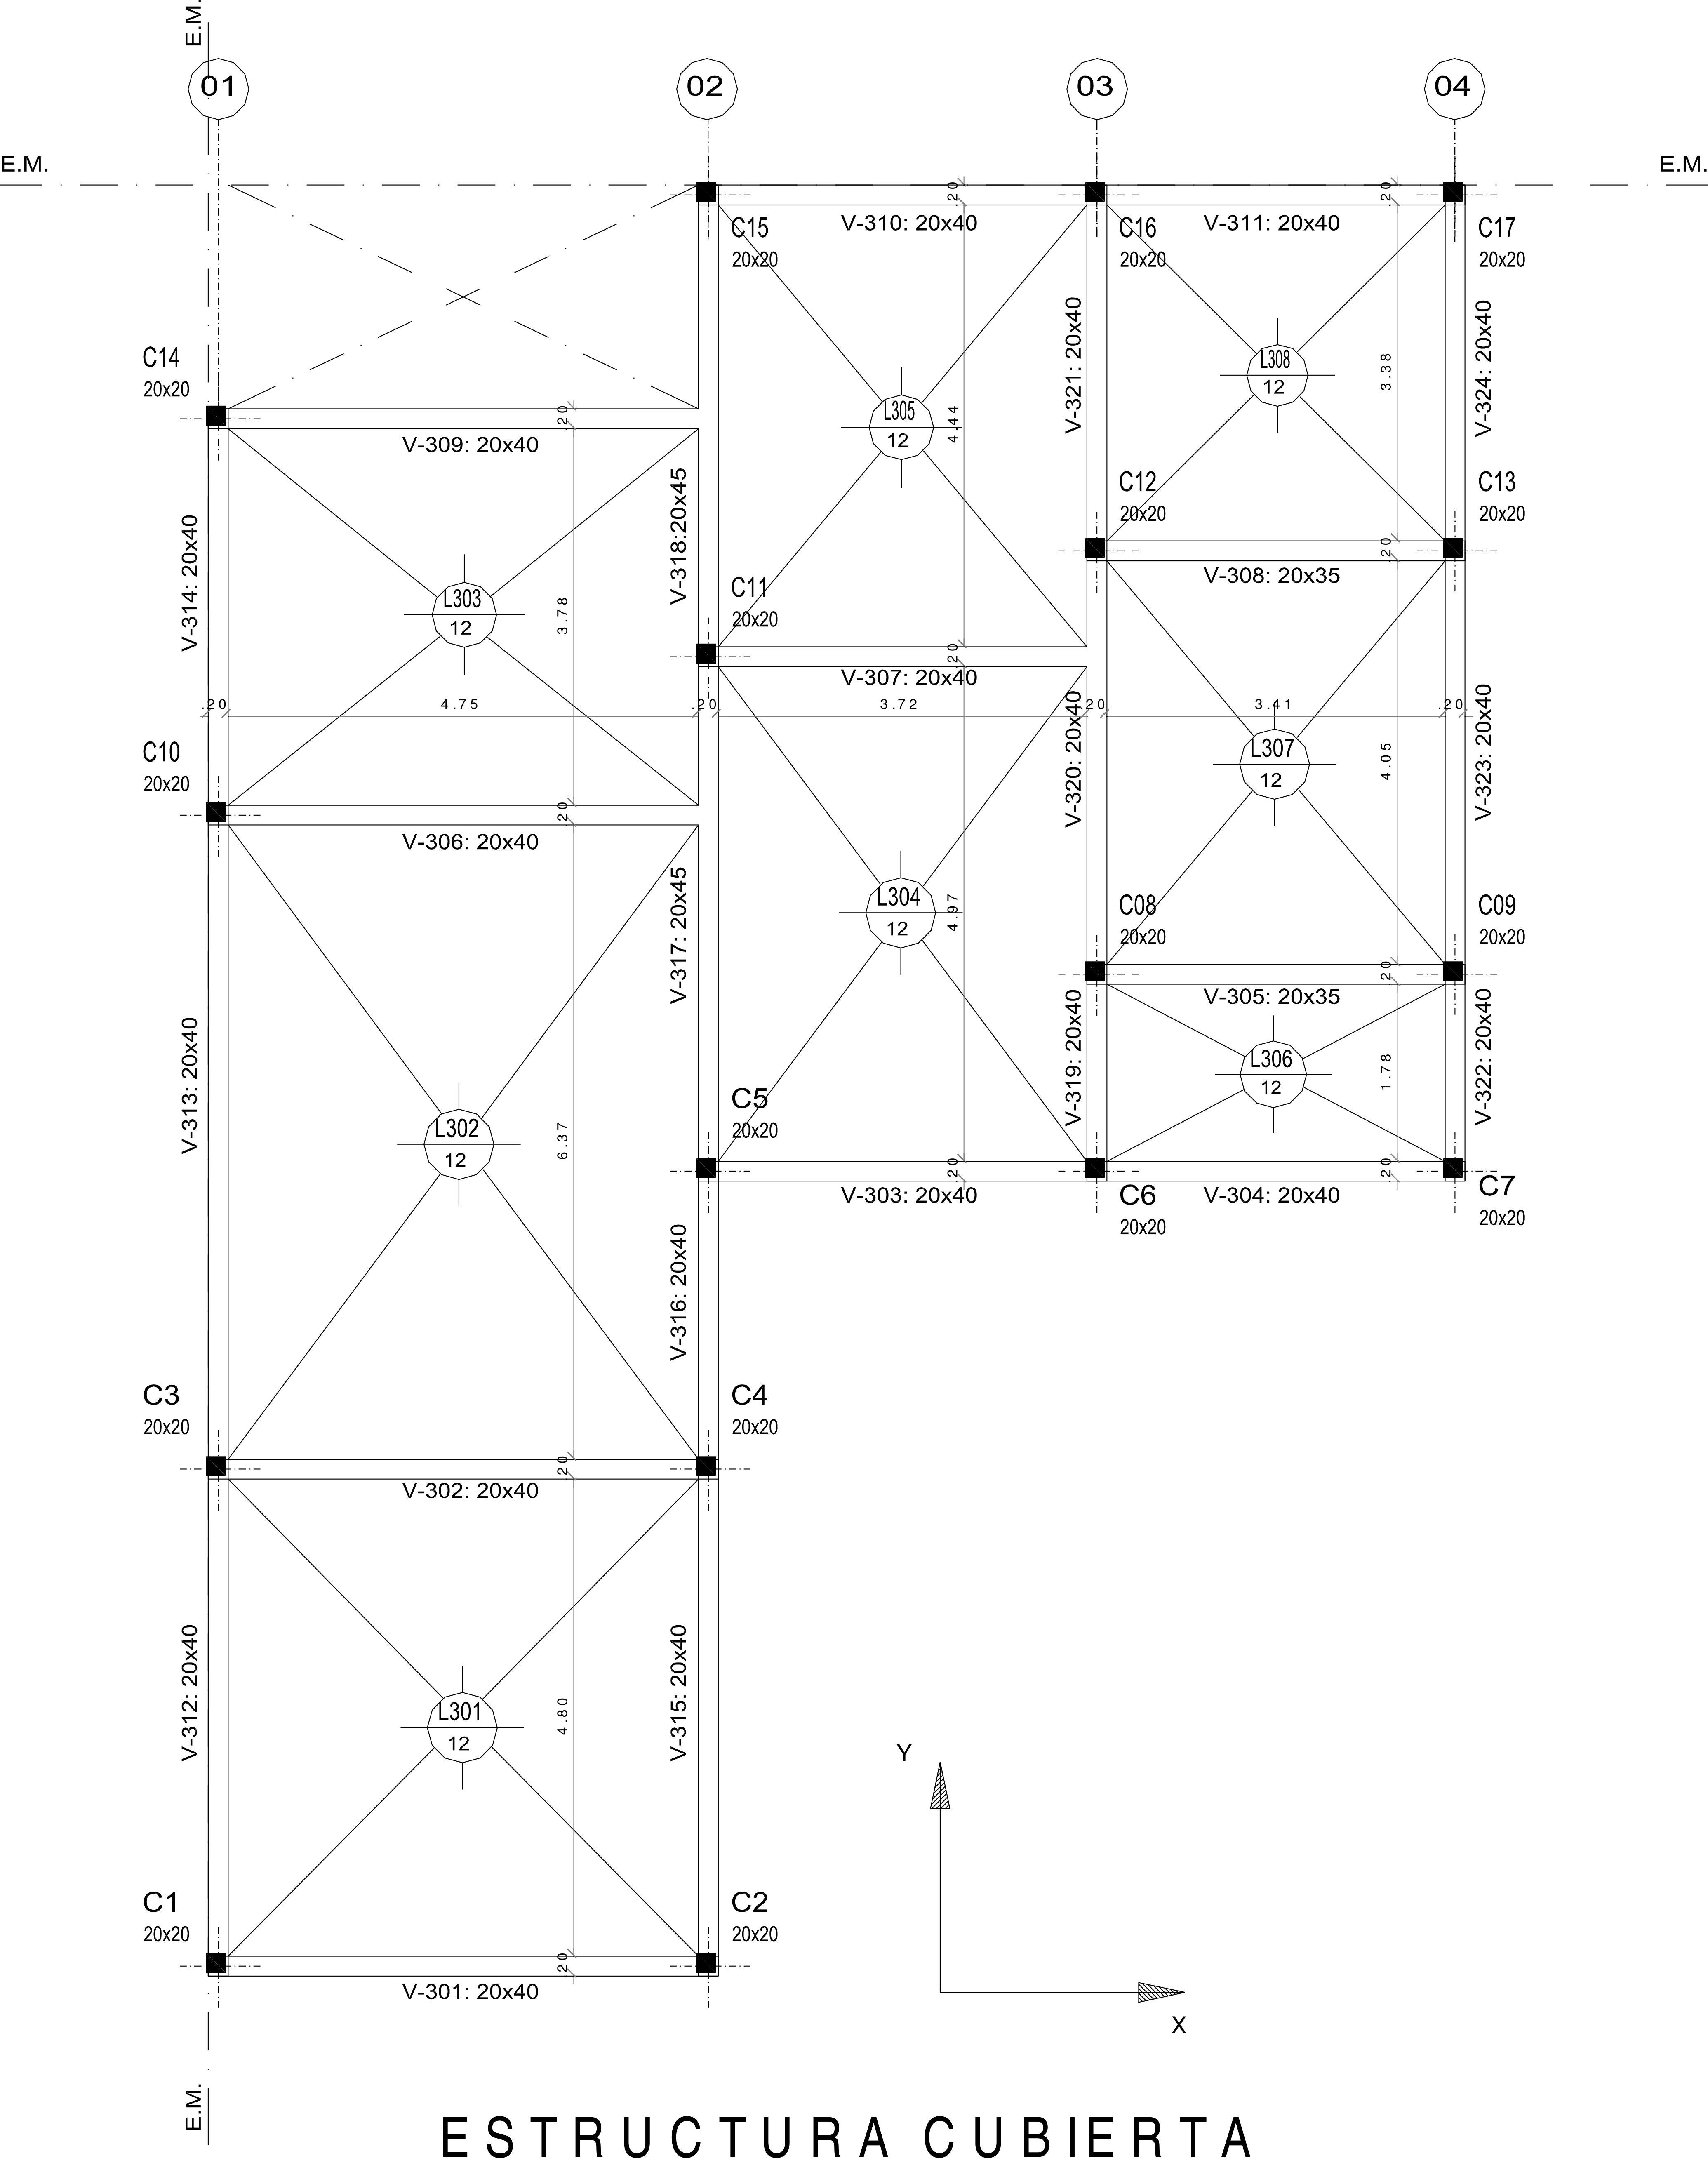
\includegraphics[scale = 0.9]{chapters/chapter_1/images/figura2.png}
\end{center}
\caption{Esquema de losas para el ejercicio 2}
\end{figure}

\begin{figure}[H]
\begin{center}
     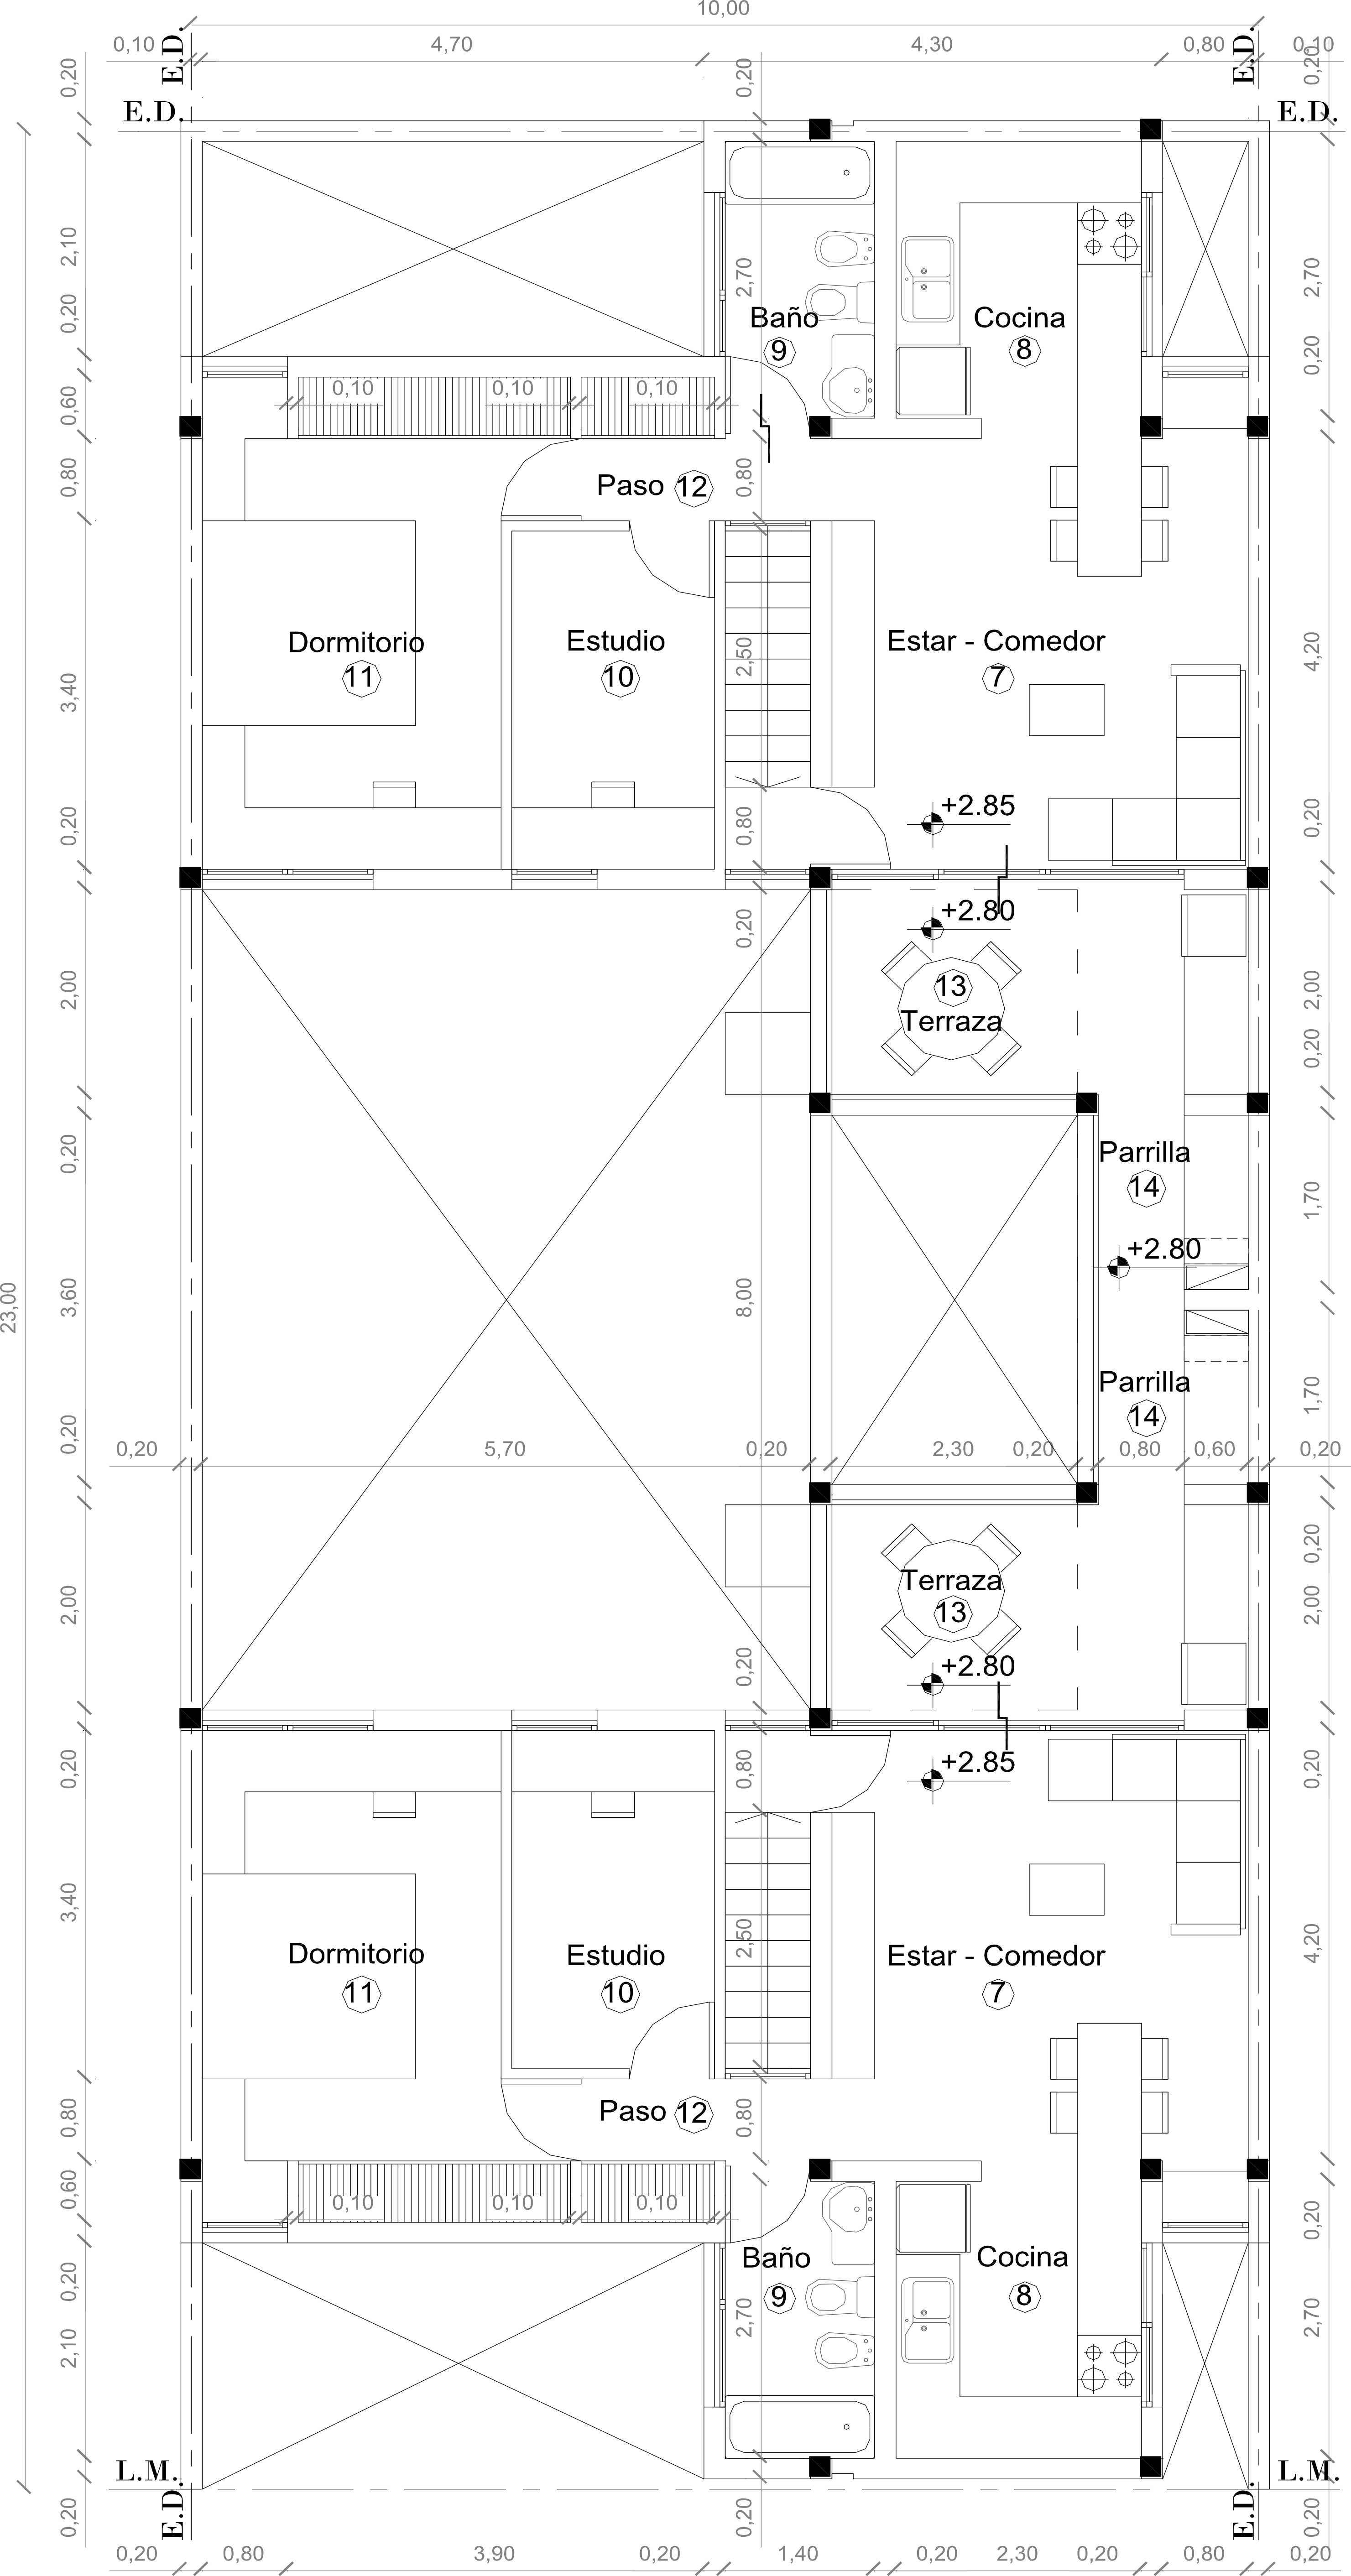
\includegraphics[scale = 0.8]{chapters/chapter_1/images/figura3.png}
\end{center}
\caption{Esquema de losas para el ejercicio 3}
\end{figure}

\end{enumerate}


\newpage
\begin{center}
\underline{\large{Solución Ejercicio 1}}
\end{center}

\begin{enumerate}
\item \underline{Sustentaciones}\\

\begin{figure}[H]
\begin{center}
     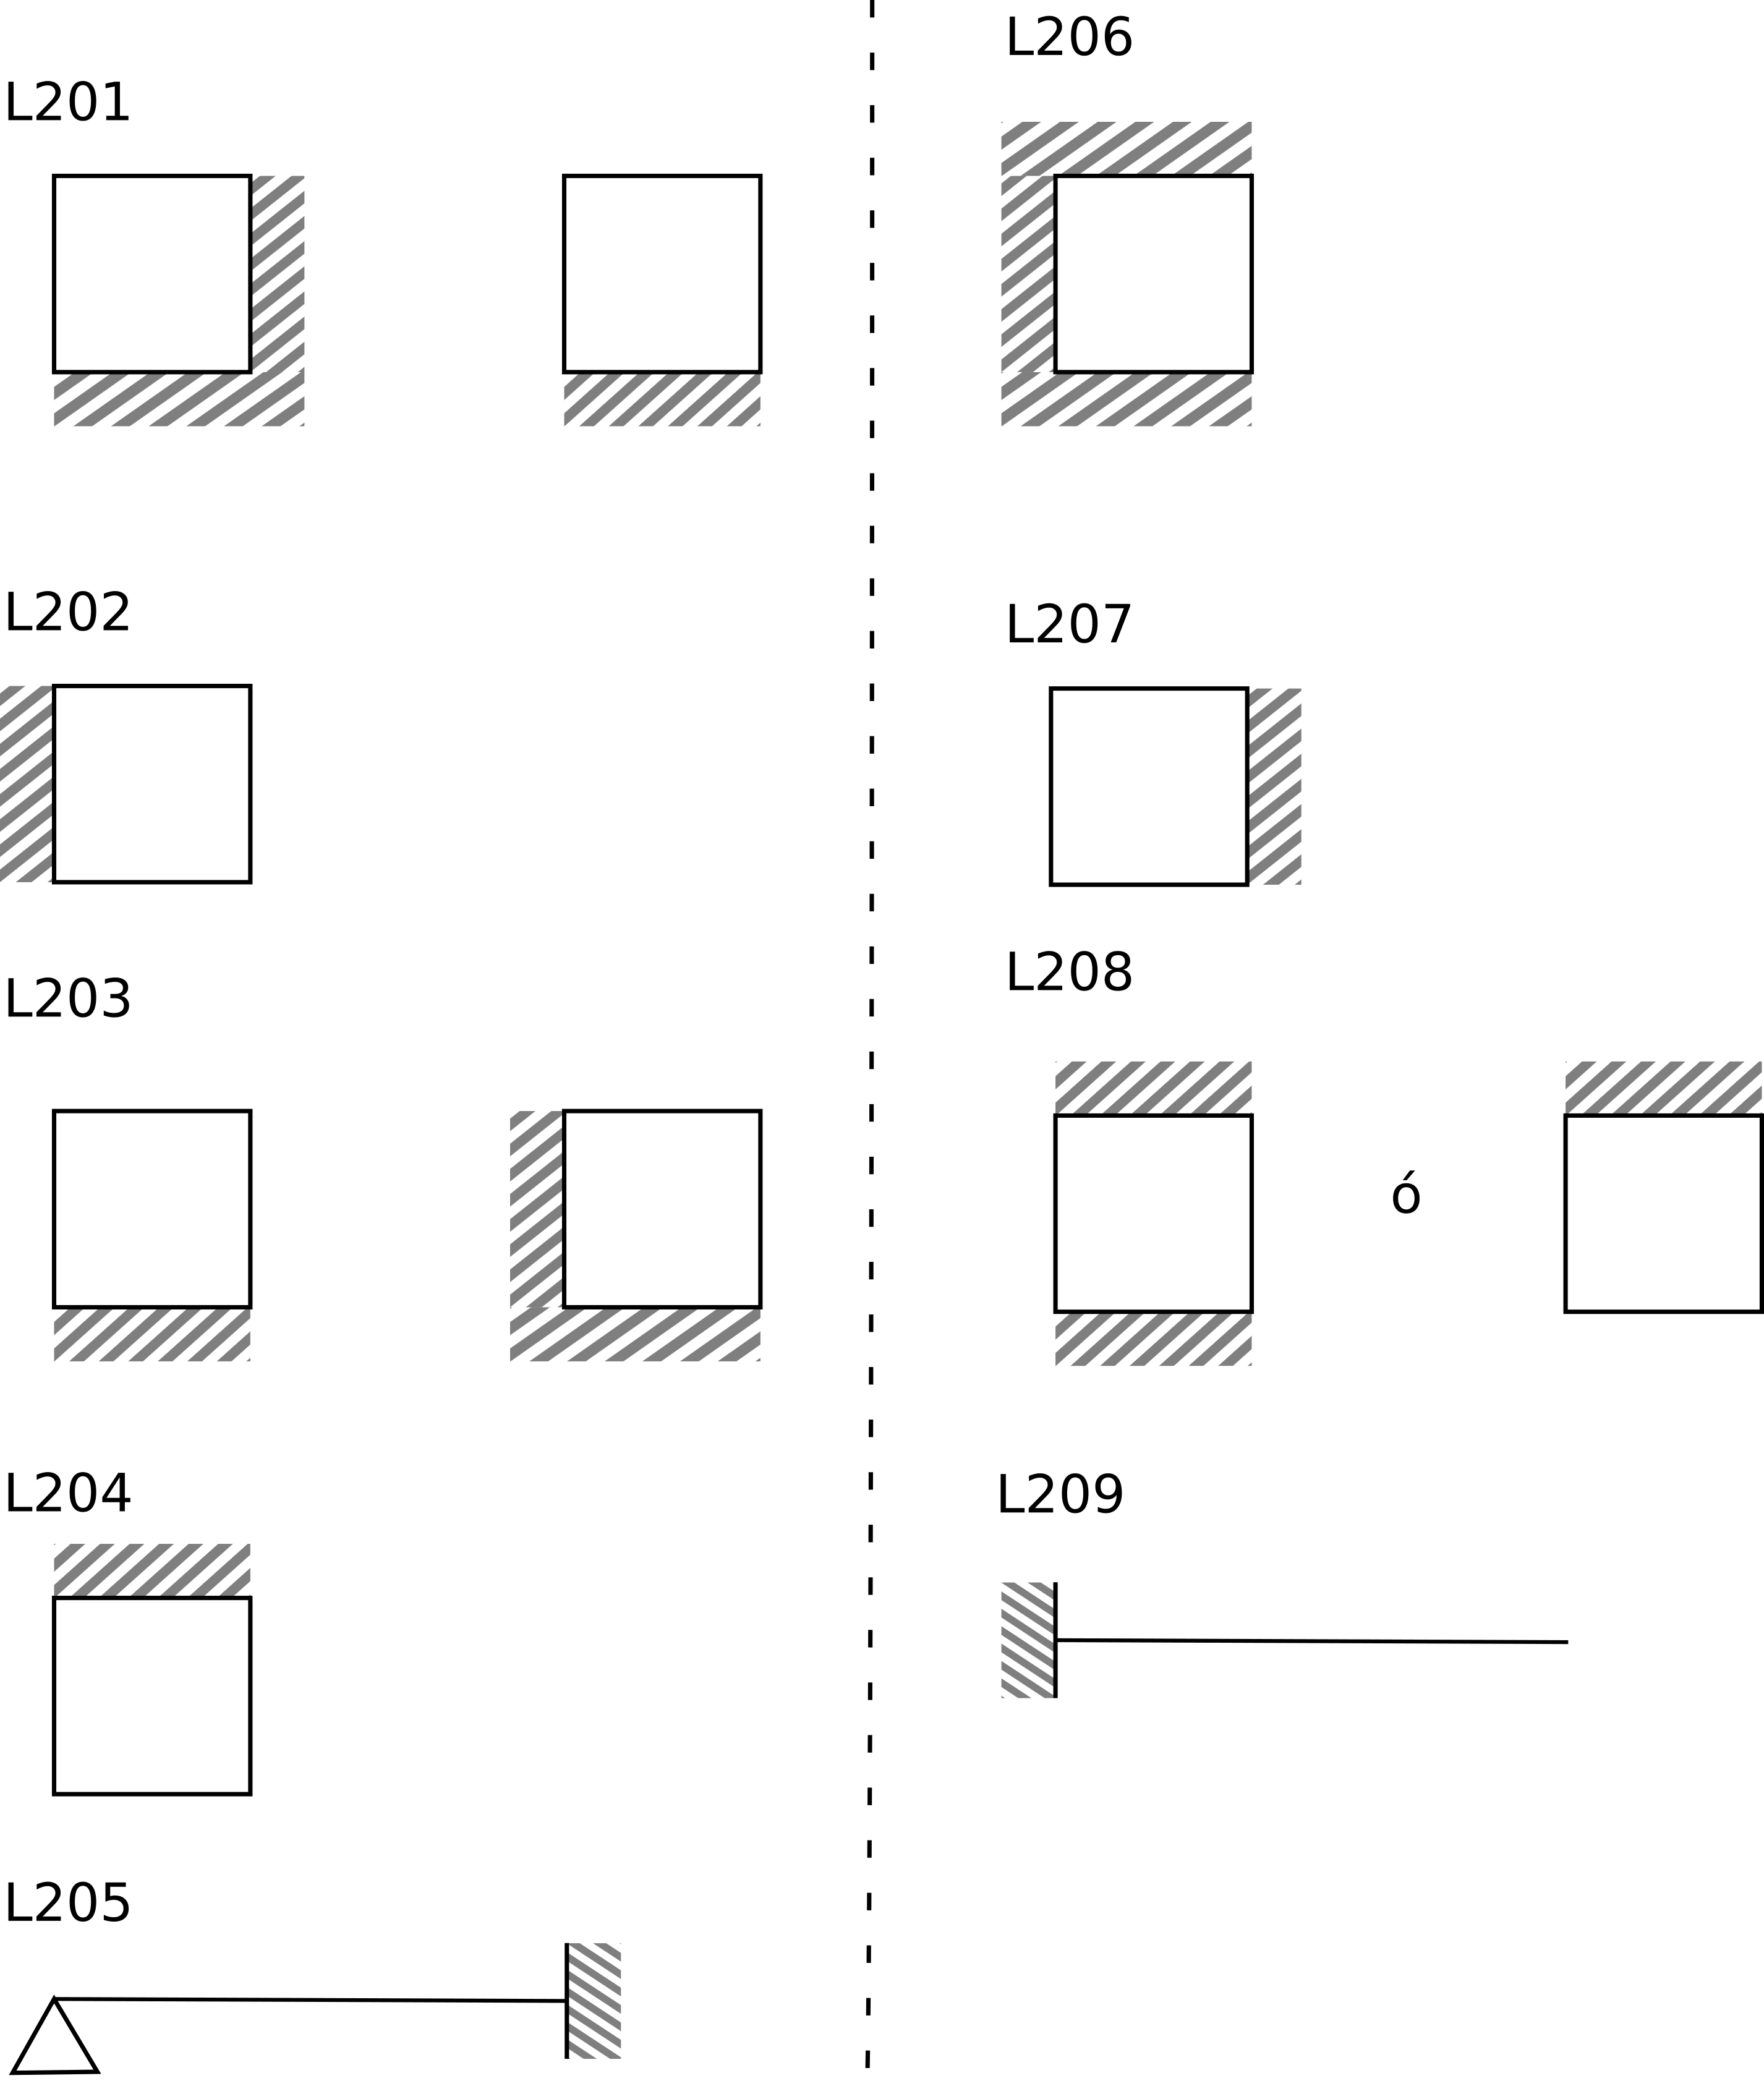
\includegraphics[scale = 1.3]{chapters/chapter_1/images/sustentacion.png}
\end{center}
\end{figure}

\newpage
\item \underline{Predimensionado de losas}\\

\begin{itemize}
\item Losa cruzada L208\\

\begin{figure}[H]
\begin{center}
     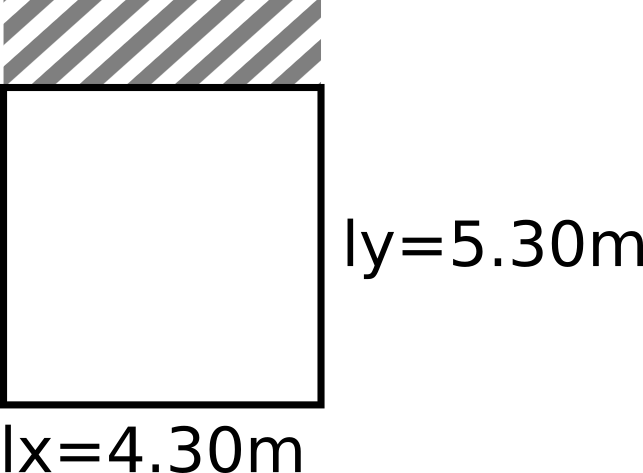
\includegraphics[scale = 1.3]{chapters/chapter_1/images/l208.png}
\end{center}
\end{figure}

\begin{center}
$l_x=4.30m$ \\
$l_y=5.30m$ \\
\end{center}

Momento de inercia de la viga.

\begin{align*}
& I_B = \frac{b \cdot h^3}{12} = \frac{20cm \cdot (50cm)^3}{12} = 208333cm^4\\
\end{align*}

Momento de inercia de la losa.

\begin{align*}
& I_{sy} = \frac{b \cdot h^3}{12} = \frac{430cm \cdot (16cm)^3}{12} = 146703cm^4\\
& I_{sx} = \frac{b \cdot h^3}{12} = \frac{530cm \cdot (16cm)^3}{12} = 180906cm^4\\
& \alpha_y = \frac{I_B}{I_{sy}} = \frac{208333cm^4}{146703cm^4} = 1.42 \\
& \alpha_x = \frac{I_B}{I_{sx}} = \frac{208333cm^4}{180906cm^4} = 1.15 \\
& \alpha_m = \frac{\alpha_x+\alpha_y}{2} = \frac{(1.15+1.42)}{2} = 1.285
\end{align*}

Dado que $0.20 < \alpha_m \leq 2 $ entonces:

\begin{align*}
& 0.20 < \alpha_m \leq 2 \\
& 0.20 < 1.285 \leq 2 \\
& h \geq = \frac{l_n \cdot (0.80+ \frac{fy}{1400})}{36+ 5 \cdot \beta \cdot (\alpha_m - 0.20)} \\
& h \geq = \frac{530cm \cdot (0.80+ \frac{420MPa}{1400})}{36+ 5 \cdot \frac{530cm}{430cm} \cdot (1.285 - 0.20)} \\
& h \geq 13.66cm \\
& h_{min} \geq 12cm
\end{align*}

Adopto $h = 16cm$ \\
$h_{adoptado} = 16 cm \geq 13.66cm$ Verifica \\

\item Losa en una dirección L209\\

\begin{figure}[H]
\begin{center}
     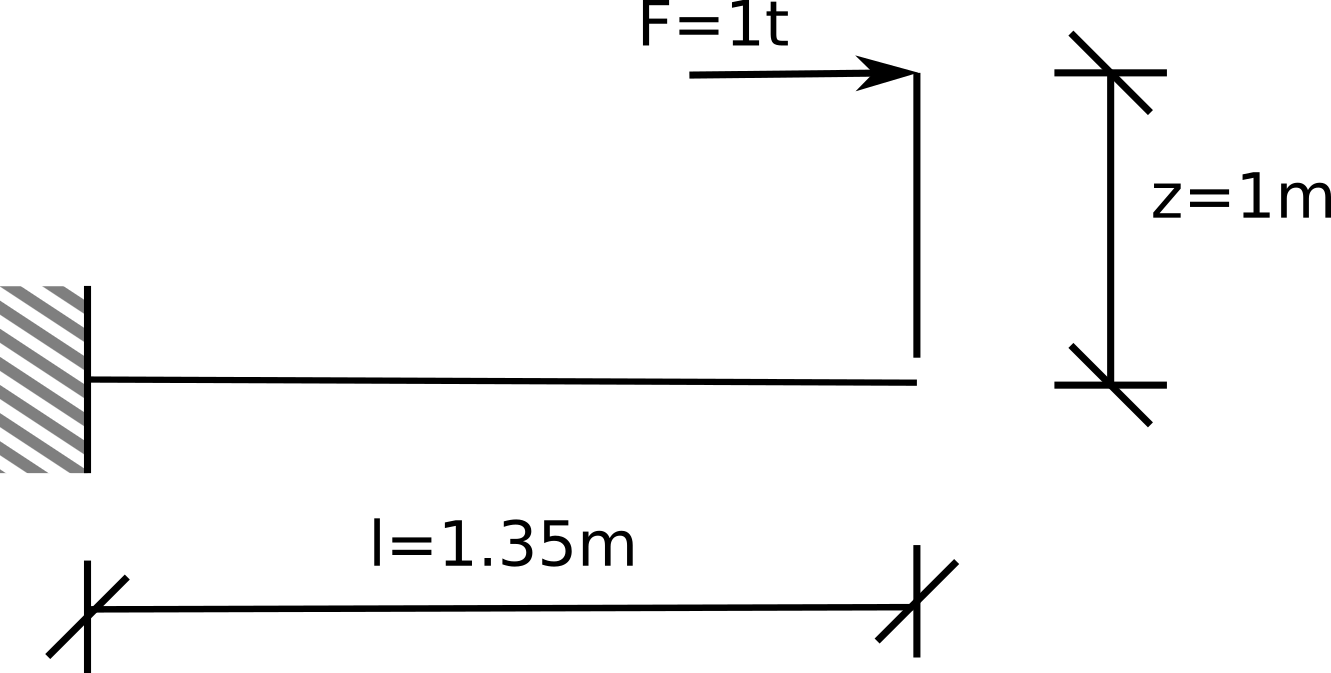
\includegraphics[scale = 1.3]{chapters/chapter_1/images/l209.png}
\end{center}
\end{figure}

$h \geq \frac{l}{10} = \frac{135cm}{10} = 13.5cm$ \\
$h_{adoptado} = 16 cm \geq 13.5cm$ Verifica
\end{itemize}

\item \underline{Análisis de cargas}\\
\begin{itemize}
\item Losa L203: Uso Sala de Reunión

\begin{align*}
& \text{Peso propio} \rightarrow 0.16m \cdot 2500 \frac{Kg}{m^3} = 400 \frac{Kg}{m^2} \Rightarrow 4 \frac{KN}{m^2} \\
& \text{Contrapiso} \rightarrow 0.07m \cdot 1600 \frac{Kg}{m^3} = 112 \frac{Kg}{m^2} \Rightarrow 1.12 \frac{KN}{m^2} \\
& \text{Cielorraso} \rightarrow 0.02m \cdot 1200 \frac{Kg}{m^3} = 24 \frac{Kg}{m^2} \Rightarrow 0.24 \frac{KN}{m^2} \\
& \text{Piso} \rightarrow 0.02m \cdot 2000 \frac{Kg}{m^3} = 40 \frac{Kg}{m^2} \Rightarrow 0.4 \frac{KN}{m^2} \\
& D = 576 \frac{Kg}{m^2} \Rightarrow 5.76 \frac{KN}{m^2} \\
& L = 500 \frac{Kg}{m^2} \Rightarrow 5 \frac{KN}{m^2} \rightarrow \text{Según CIRSOC 101-05 - Capítulo 9}\\
& q_u = 1.2 \cdot D + 1.6 \cdot L = 1.2 \cdot 576 \frac{Kg}{m^2} + 1.6 \cdot 500 \frac{Kg}{m^2} = 1492 \frac{Kg}{m^2} \Rightarrow \framebox{$14.92 \frac{KN}{m^2}$} \\
& q_u = 1.4 \cdot D = 1.4 \cdot 576 \frac{Kg}{m^2} = 806 \frac{Kg}{m^2} \Rightarrow 8.06 \frac{KN}{m^2}
\end{align*}

\newpage
\item Losa L206: Uso Archivo / Depósito

\begin{align*}
& \text{Peso propio} \rightarrow 0.16m \cdot 2500 \frac{Kg}{m^3} = 400 \frac{Kg}{m^2} \Rightarrow 4 \frac{KN}{m^2} \\
& \text{Contrapiso} \rightarrow 0.07m \cdot 1600 \frac{Kg}{m^3} = 112 \frac{Kg}{m^2} \Rightarrow 1.12 \frac{KN}{m^2} \\
& \text{Cielorraso} \rightarrow 0.02m \cdot 1200 \frac{Kg}{m^3} = 24 \frac{Kg}{m^2} \Rightarrow 0.24 \frac{KN}{m^2} \\
& \text{Piso} \rightarrow 0.02m \cdot 2000 \frac{Kg}{m^3} = 40 \frac{Kg}{m^2} \Rightarrow 0.4 \frac{KN}{m^2} \\
& D = 576 \frac{Kg}{m^2} \Rightarrow 5.76 \frac{KN}{m^2} \\
& L = 700 \frac{Kg}{m^2} \Rightarrow 7 \frac{KN}{m^2} \rightarrow \text{Según CIRSOC 101-05 - Capítulo 9}\\
& Dpared = \frac{2 \cdot (0.15m \cdot 3m \cdot 1.35m \cdot 1700 \frac{Kg}{m^3}) \cdot 1.50}{5.15m \cdot 4.3m} = 140 \frac{Kg}{m^2} \\
& Dtotal = D + Dpared = 576 \frac{Kg}{m^2} + 140 \frac{Kg}{m^2} = 716 \frac{Kg}{m^2} \\
& q_u = 1.2 \cdot D + 1.6 \cdot L = 1.2 \cdot 716 \frac{Kg}{m^2} + 1.6 \cdot 700 \frac{Kg}{m^2} = 1980 \frac{Kg}{m^2} \Rightarrow \framebox{$19.80 \frac{KN}{m^2}$} \\
& q_u = 1.4 \cdot D = 1.4 \cdot 716 \frac{Kg}{m^2} = 1002 \frac{Kg}{m^2} \Rightarrow 10.02 \frac{KN}{m^2}
\end{align*}

\item Losa L208: Uso Archivo

\begin{align*}
& \text{Peso propio} \rightarrow 0.16m \cdot 2500 \frac{Kg}{m^3} = 400 \frac{Kg}{m^2} \Rightarrow 4 \frac{KN}{m^2} \\
& \text{Contrapiso} \rightarrow 0.07m \cdot 1600 \frac{Kg}{m^3} = 112 \frac{Kg}{m^2} \Rightarrow 1.12 \frac{KN}{m^2} \\
& \text{Cielorraso} \rightarrow 0.02m \cdot 1200 \frac{Kg}{m^3} = 24 \frac{Kg}{m^2} \Rightarrow 0.24 \frac{KN}{m^2} \\
& \text{Piso} \rightarrow 0.02m \cdot 2000 \frac{Kg}{m^3} = 40 \frac{Kg}{m^2} \Rightarrow 0.4 \frac{KN}{m^2} \\
& D = 576 \frac{Kg}{m^2} \Rightarrow 5.76 \frac{KN}{m^2} \\
& L = 700 \frac{Kg}{m^2} \Rightarrow 7 \frac{KN}{m^2} \rightarrow \text{Según CIRSOC 101-05 - Capítulo 9}\\
& Dpared = \frac{(0.10m \cdot 3m \cdot 4.30m \cdot 1700 \frac{Kg}{m^3}) \cdot 1.50}{4.30m \cdot 5.30m} = 144 \frac{Kg}{m^2} \\
& Dtotal = D + Dpared = 576 \frac{Kg}{m^2} + 144 \frac{Kg}{m^2} = 720 \frac{Kg}{m^2} \\
& q_u = 1.2 \cdot D + 1.6 \cdot L = 1.2 \cdot 720 \frac{Kg}{m^2} + 1.6 \cdot 700 \frac{Kg}{m^2} = 1984 \frac{Kg}{m^2} \Rightarrow \framebox{$19.84 \frac{KN}{m^2}$} \\
& q_u = 1.4 \cdot D = 1.4 \cdot 720 \frac{Kg}{m^2} = 1008 \frac{Kg}{m^2} \Rightarrow 10.08 \frac{KN}{m^2}
\end{align*}

\newpage
\item Losa L209: Uso Balcón

\begin{align*}
& \text{Peso propio} \rightarrow 0.16m \cdot 2500 \frac{Kg}{m^3} = 400 \frac{Kg}{m^2} \Rightarrow 4 \frac{KN}{m^2} \\
& \text{Contrapiso} \rightarrow 0.07m \cdot 1600 \frac{Kg}{m^3} = 112 \frac{Kg}{m^2} \Rightarrow 1.12 \frac{KN}{m^2} \\
& \text{Cielorraso} \rightarrow 0.02m \cdot 1200 \frac{Kg}{m^3} = 24 \frac{Kg}{m^2} \Rightarrow 0.24 \frac{KN}{m^2} \\
& \text{Piso} \rightarrow 0.02m \cdot 2000 \frac{Kg}{m^3} = 40 \frac{Kg}{m^2} \Rightarrow 0.4 \frac{KN}{m^2} \\
& D = 576 \frac{Kg}{m^2} \Rightarrow 5.76 \frac{KN}{m^2} \\
& L = 500 \frac{Kg}{m^2} \Rightarrow 5 \frac{KN}{m^2} \rightarrow \text{Según CIRSOC 101-05 - Capítulo 9}\\
& q_u = 1.2 \cdot D + 1.6 \cdot L = 1.2 \cdot 576 \frac{Kg}{m^2} + 1.6 \cdot 500 \frac{Kg}{m^2} = 1491 \frac{Kg}{m^2} \Rightarrow \framebox{$14.91 \frac{KN}{m^2}$} \\
& q_u = 1.4 \cdot D = 1.4 \cdot 576 \frac{Kg}{m^2} = 806 \frac{Kg}{m^2} \Rightarrow 8.06 \frac{KN}{m^2}
\end{align*}

\end{itemize}


\item \underline{Momentos flectores}\\

\begin{itemize}
\item Losa L203

\begin{figure}[H]
\begin{center}
     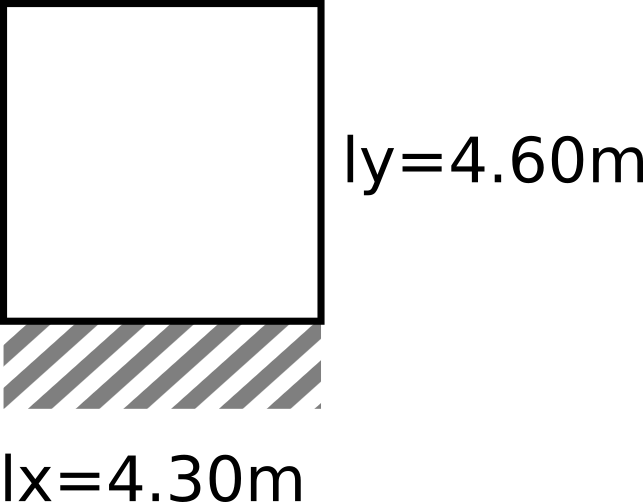
\includegraphics[scale = 1.3]{chapters/chapter_1/images/l203.png}
\end{center}
\end{figure}


\begin{align*}
& \frac{l_x}{l_y} = \frac{4.30m}{4.60m} = 0.93 \rightarrow \text{cambio de ejes} \quad \frac{l'_y}{l'_x} = 0.93\\
& m'_{xe} = 11.35 \rightarrow m_{ye} = 11.35 \\
& m'_x = 30.58 \rightarrow m_y = 30.58 \\
& m'_y= 35.46 \rightarrow m_x = 35.46 \\
& Mu_{ye} = \frac{U \cdot (lmenor)^2}{m_{ye}} = \frac{1.492 \frac{t}{m^2} \cdot (4.30m)^2}{11.35} = 2.43 \frac{t \cdot m}{m} \\
& Mu_y = \frac{U \cdot (lmenor)^2}{m_y} = \frac{1.492 \frac{t}{m^2} \cdot (4.30m)^2}{30.58} = 0.9 \frac{t \cdot m}{m} \\
& Mu_x = \frac{U \cdot (lmenor)^2}{m_x} = \frac{1.492 \frac{t}{m^2} \cdot (4.30m)^2}{35.46} = 0.78 \frac{t \cdot m}{m}
\end{align*}

\newpage
\item Losa L206 \\
El empotramiento de la izquierda es eliminado debido a que no compatibilizan con las losas L206 y L207.

\begin{figure}[H]
\begin{center}
     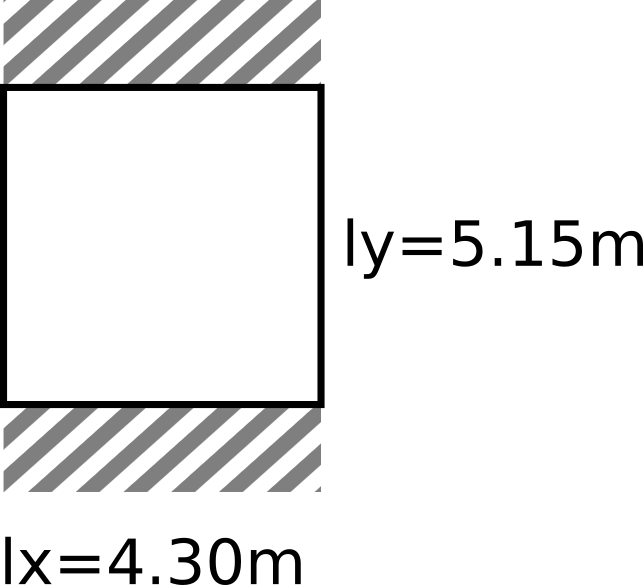
\includegraphics[scale = 1.3]{chapters/chapter_1/images/l206.png}
\end{center}
\end{figure}

\begin{align*}
& \frac{l_x}{l_y} = \frac{4.30m}{5.15m} = 0.83 \rightarrow \text{cambio de ejes} \quad \frac{l'_y}{l'_x} = 0.83\\
& m'_{xe} = 11.78 \rightarrow m_{ye} = 11.78 \\
& m'_x = 31.85 \rightarrow m_y = 31.85 \\
& m'_y= 37.45 \rightarrow m_x = 37.45 \\
& Mu_{ye} = \frac{U \cdot (lmenor)^2}{m_{ye}} = \frac{1.98 \frac{t}{m^2} \cdot (4.30m)^2}{11.78} = 3.11 \frac{t \cdot m}{m} \\
& Mu_y = \frac{U \cdot (lmenor)^2}{m_y} = \frac{1.98 \frac{t}{m^2} \cdot (4.30m)^2}{31.85} = 1.15 \frac{t \cdot m}{m} \\
& Mu_x = \frac{U \cdot (lmenor)^2}{m_x} = \frac{1.98 \frac{t}{m^2} \cdot (4.30m)^2}{37.45} = 0.98 \frac{t \cdot m}{m}
\end{align*}

\item Losa L208

\begin{figure}[H]
\begin{center}
     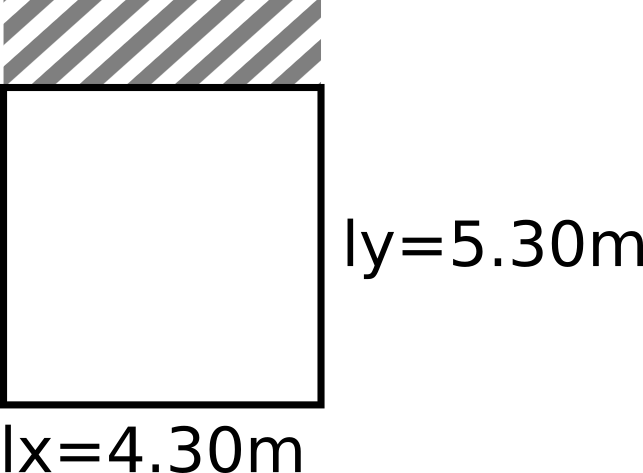
\includegraphics[scale = 1.3]{chapters/chapter_1/images/l208.png}
\end{center}
\end{figure}

\begin{align*}
& \frac{l_x}{l_y} = \frac{4.30m}{5.30m} = 0.80 \rightarrow \text{cambio de ejes} \quad \frac{l'_y}{l'_x} = 0.80\\
& m'_{xe} = 9.89 \rightarrow m_{ye} = 9.89 \\
& m'_x = 30.86 \rightarrow m_y = 30.86 \\
& m'_y= 23.64 \rightarrow m_x = 23.64 \\
& Mu_{ye} = \frac{U \cdot (lmenor)^2}{m_{ye}} = \frac{1.984 \frac{t}{m^2} \cdot (4.30m)^2}{9.89} = 3.71 \frac{t \cdot m}{m} \\
& Mu_y = \frac{U \cdot (lmenor)^2}{m_y} = \frac{1.984 \frac{t}{m^2} \cdot (4.30m)^2}{30.86} = 1.19 \frac{t \cdot m}{m} \\
& Mu_x = \frac{U \cdot (lmenor)^2}{m_x} = \frac{1.984 \frac{t}{m^2} \cdot (4.30m)^2}{23.64} = 1.55 \frac{t \cdot m}{m}
\end{align*}

\newpage
\item Losa L209

\begin{figure}[H]
\begin{center}
     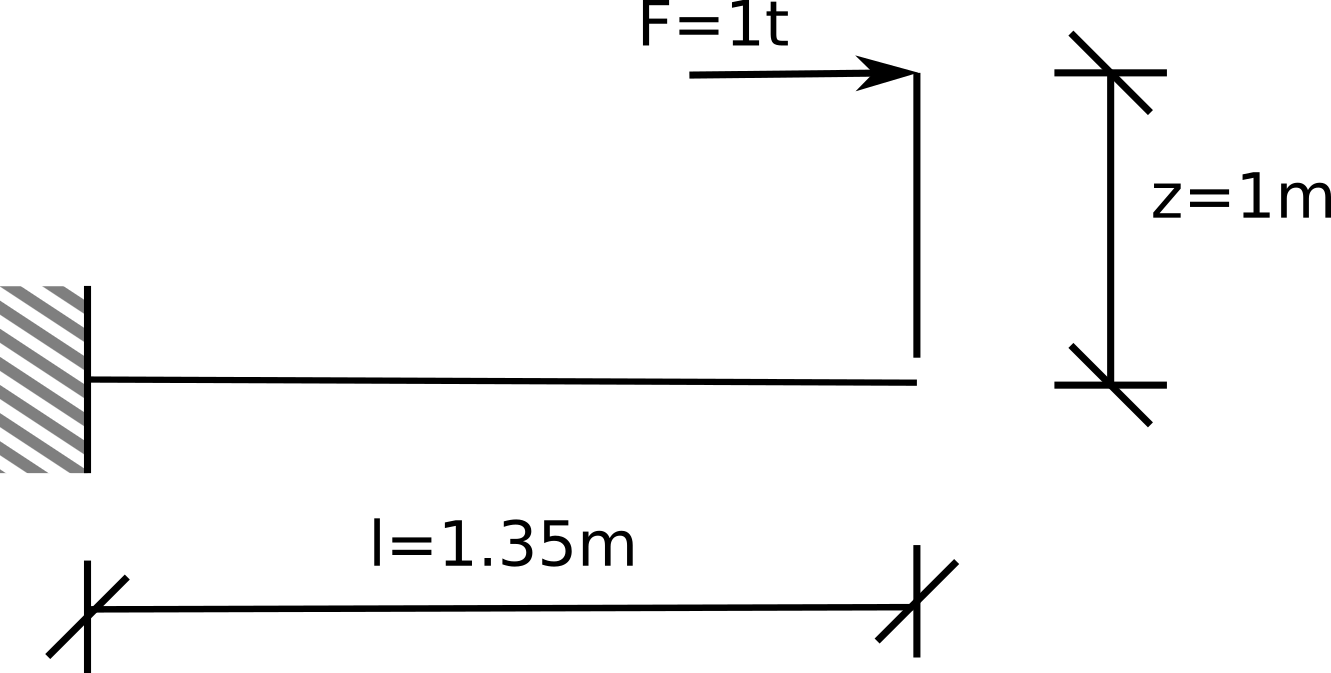
\includegraphics[scale = 1.3]{chapters/chapter_1/images/l209.png}
\end{center}
\end{figure}

\begin{align*}
& Mu_{ye} = \frac{U \cdot l^2}{2} + F \cdot z = \frac{1.491 \frac{t}{m^2} \cdot (1.35m)^2}{2} + 0.1t \cdot 1m = 1.46 \frac{t \cdot m}{m}
\end{align*}

\end{itemize}

\newpage
\item \underline{Compatibilización de Momentos}\\

\begin{figure}[H]
\begin{center}
     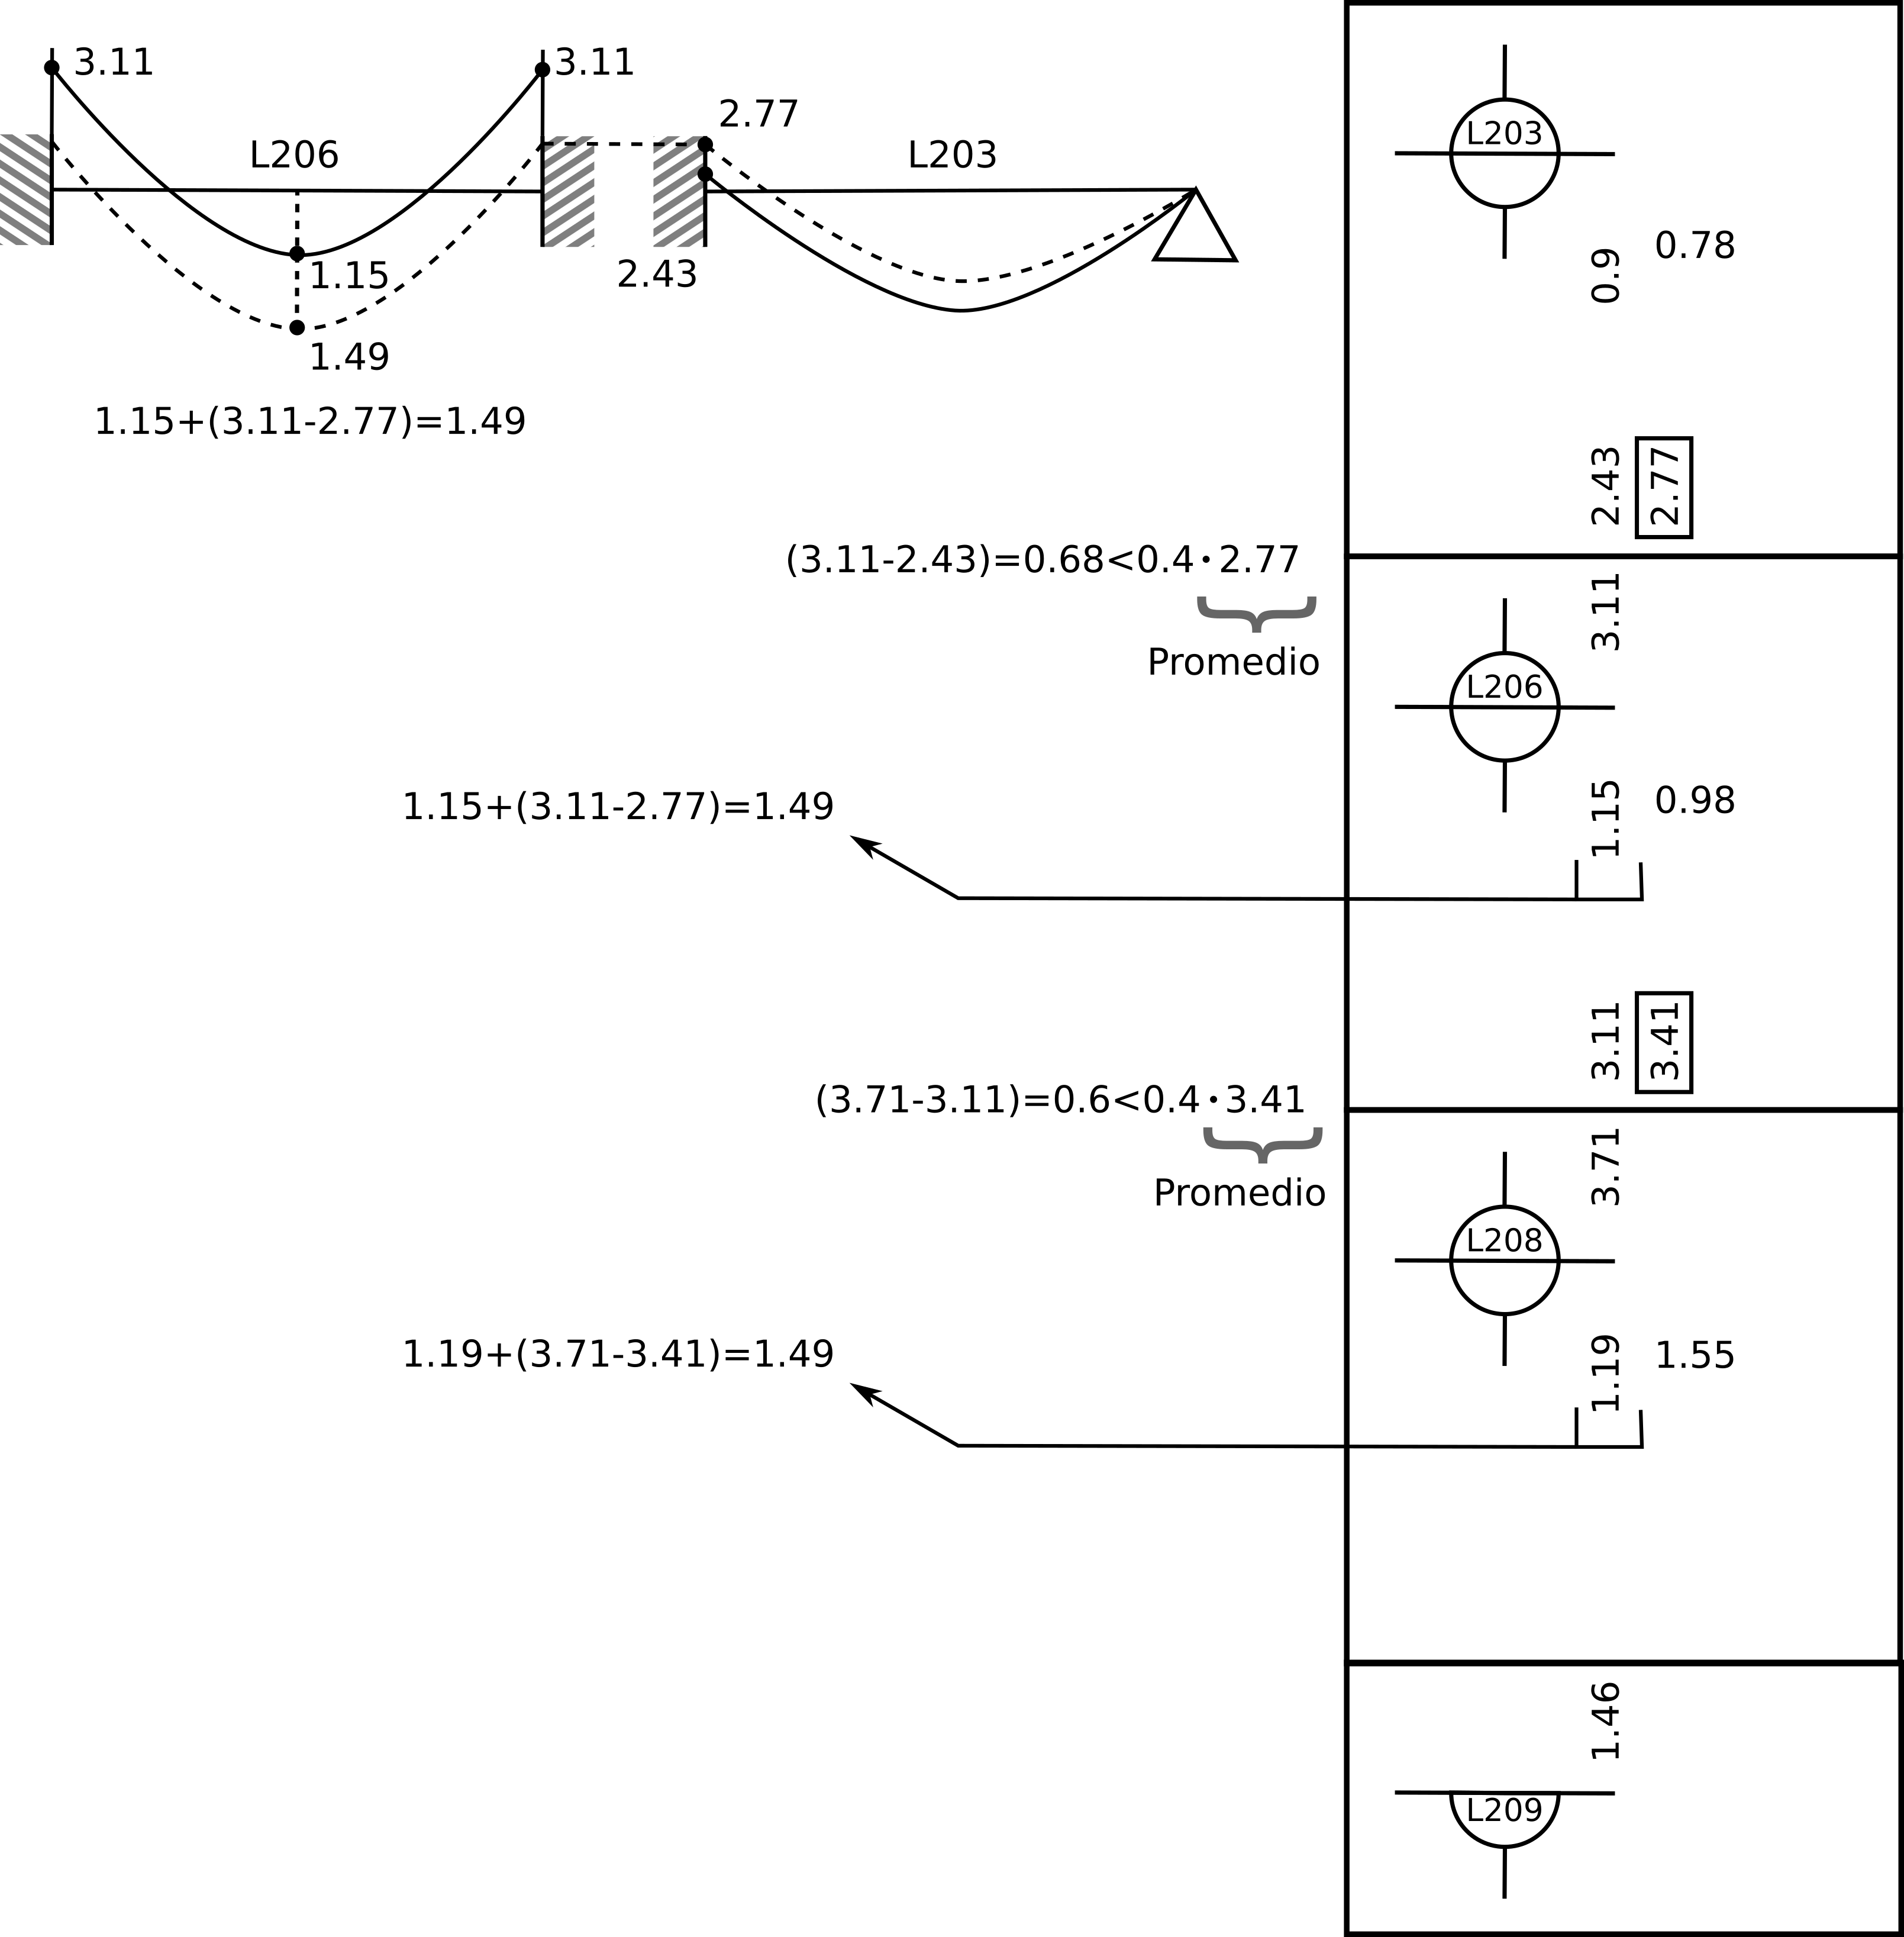
\includegraphics[scale = 1.3]{chapters/chapter_1/images/compatibilidad.png}
\end{center}
\end{figure}

\newpage
\item \underline{Cálculo de Armaduras}\\
\begin{itemize}
\item Armadura Superior

\begin{align*}
& M_u = 3.41 \frac{t \cdot m}{m} \\
& M_n = \frac{M_u}{\phi} = \frac{3.41 \frac{t \cdot m}{m}}{0.9} = 3.79 \frac{t \cdot m}{m} \Rightarrow 0.0379 \frac{MN \cdot m}{m} \\
& d = h -db - Cc = 16cm - 1cm - 2cm = 13cm \\
& Kd = \frac{d}{\sqrt[]{\frac{M_n}{b}}} = \frac{0.13m}{\sqrt[]{\frac{0.0379 \frac{MN \cdot m}{m}}{1m}}} = 0.66 \Rightarrow Ke = 25.207 \\
& A_s = Ke \cdot \frac{M_n}{d} = 25.207 \cdot \frac{0.0379 \frac{MN \cdot m}{m}}{0.13m} = 7.35 \frac{cm^2}{m}\\
& As_{min} = 0.0018 \cdot b \cdot h = 0.0018 \cdot 100cm \cdot 16cm = 2.88 \frac{cm^2}{m}
\end{align*}

Se adopta A° superior $\phi$ 10 cada 10cm $\rightarrow \framebox{$7.85 \frac{cm^2}{m}$}$ \\

\underline{Verificación de separaciones}\\

\[ s = 10cm \leq \left\{ \begin{array}{ll}
         2.5 \cdot h = 2.5 \cdot 16cm = 40cm \quad \surd & \\
         25 \cdot db = 25 \cdot 1cm = 25cm \quad \surd &\\
         30cm \quad \surd & \end{array} \right. \] 
         
\[ s =10cm \geq \left\{ \begin{array}{ll}
         db = 1cm \quad \surd & \\
         \geq 2.5cm \quad \surd &\\
         \geq \frac{4}{3} \cdot \text{Tamaño máximo del agregado} & \end{array} \right. \] 

\item Armadura Inferior

\begin{align*}
& M_u = 1.55 \frac{t \cdot m}{m} \\
& M_n = \frac{M_u}{\phi} = \frac{1.55 \frac{t \cdot m}{m}}{0.9} = 1.71 \frac{t \cdot m}{m} \Rightarrow 0.0171 \frac{MN \cdot m}{m} \\
& d = h -db - Cc - \frac{db}{2}= 16cm - 1cm - 2cm - \frac{1cm}{2}= 12.5cm \\
& Kd = \frac{d}{\sqrt[]{\frac{M_n}{b}}} = \frac{0.125m}{\sqrt[]{\frac{0.0171 \frac{MN \cdot m}{m}}{1m}}} = 0.956 \Rightarrow Ke = 24.49 \\
& A_s = Ke \cdot \frac{M_n}{d} = 24.49 \cdot \frac{0.0171 \frac{MN \cdot m}{m}}{0.125m} = 3.35 \frac{cm^2}{m}\\
& As_{min} = 0.0018 \cdot b \cdot h = 0.0018 \cdot 100cm \cdot 16cm = 2.88 \frac{cm^2}{m}
\end{align*}

Se adopta A° inferior $\phi$ 8 cada 15cm $\rightarrow \framebox{$3.36 \frac{cm^2}{m}$}$ \\

\newpage
\underline{Verificación de separaciones}\\

\[ s = 15cm \leq \left\{ \begin{array}{ll}
         2.5 \cdot h = 2.5 \cdot 16cm = 40cm \quad \surd & \\
         25 \cdot db = 25 \cdot 0.8cm = 20cm \quad \surd &\\
         30cm \quad \surd & \end{array} \right. \] 
         
\[ s =15cm \geq \left\{ \begin{array}{ll}
         db = 0.8cm \quad \surd & \\
         \geq 2.5cm \quad \surd &\\
         \geq \frac{4}{3} \cdot \text{Tamaño máximo del agregado} & \end{array} \right. \] 

\item Cálculo de Armadura para el orificio \\

Dado un orificio cuadrado de 1.30m de lado, se requiere realizar su armado, para ello debemos compensar la sección de acero que se ha quitado respecto a si tuviesemos la losa completa.\\
Estimamos la cantidad de barras sabiendo que tenemos una Armadura Inferior con $\phi$ 8 cada 15cm.\\

Cantidad de barras $ = \frac{Lado}{Separacion}+1 = \frac{1.30m}{0.15m} + 1 = 9.7 \Rightarrow 10 \quad barras$\\

10 barras del $\phi$ 8 representan una sección de $5.03cm^2$ para cubrirlas adoptamos 3 barras $\phi$ 12 superior e inferior totalizando una sección de $6.79cm^2$\\

La longitud de anclaje de las barras que llegan al perimetro del orificio se estiman en $2 \cdot h = 2 \cdot 16cm = 32cm$\\

\begin{figure}[H]
\begin{center}
     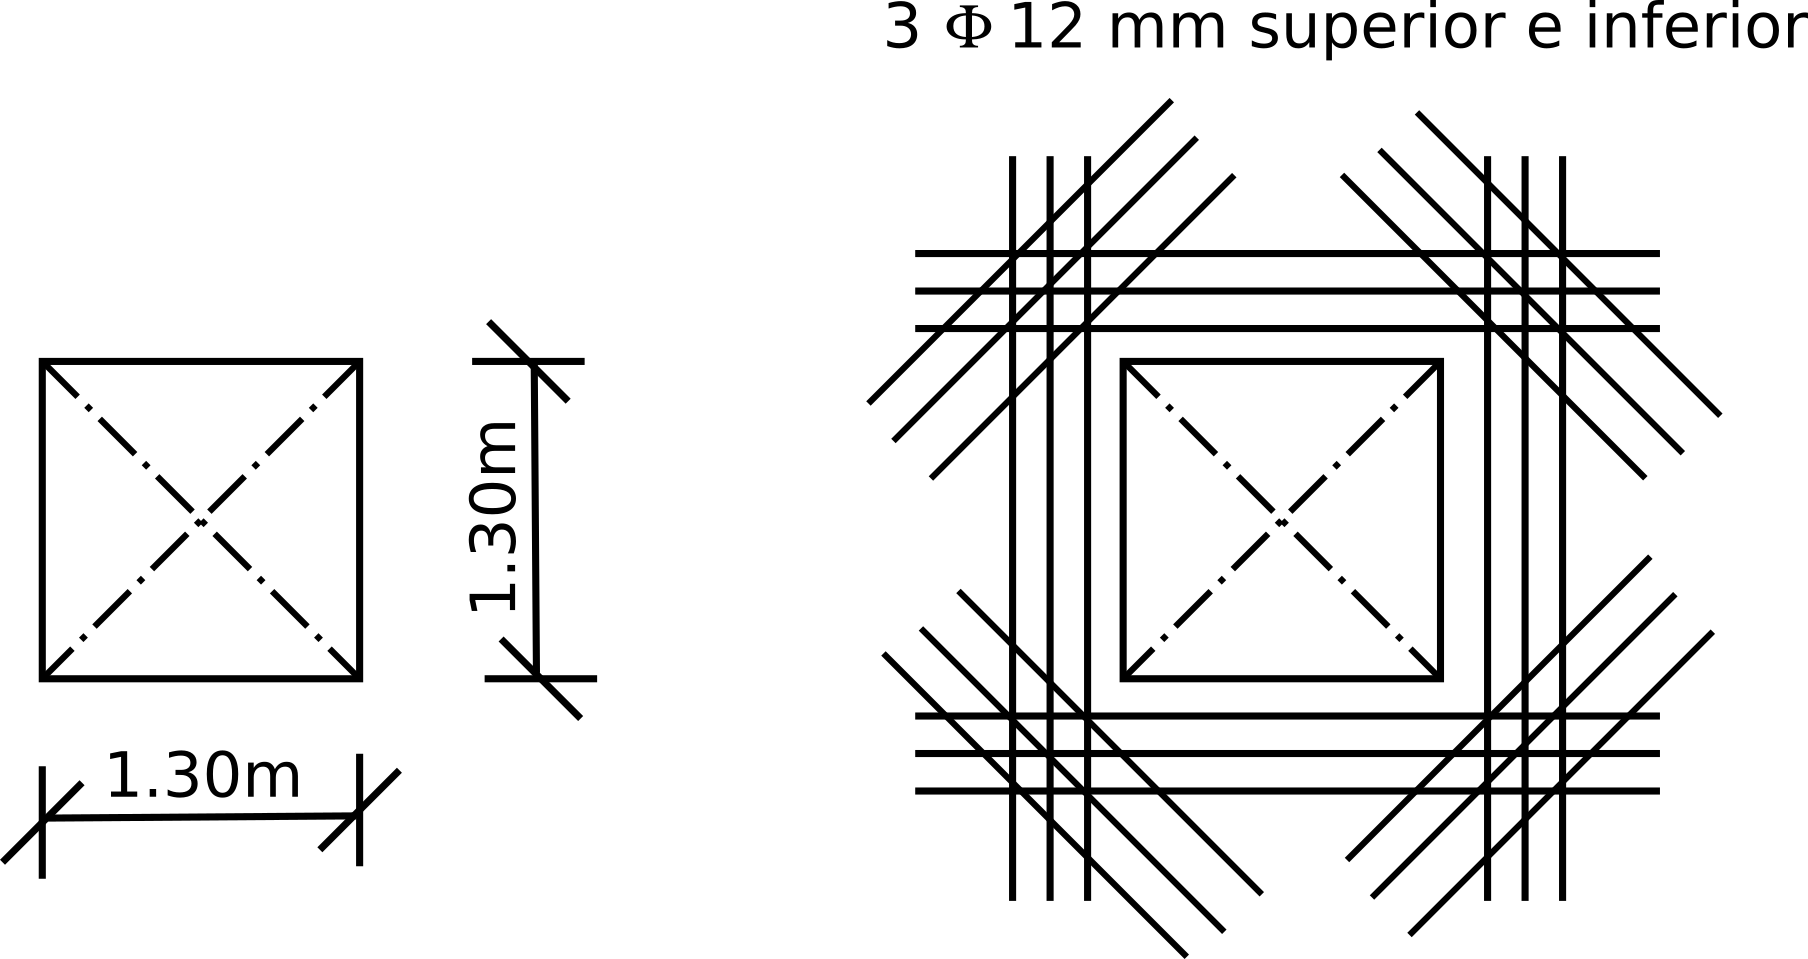
\includegraphics[scale = 1.2]{chapters/chapter_1/images/orificio1.png}
\end{center}
\end{figure}

\begin{figure}[H]
\begin{center}
     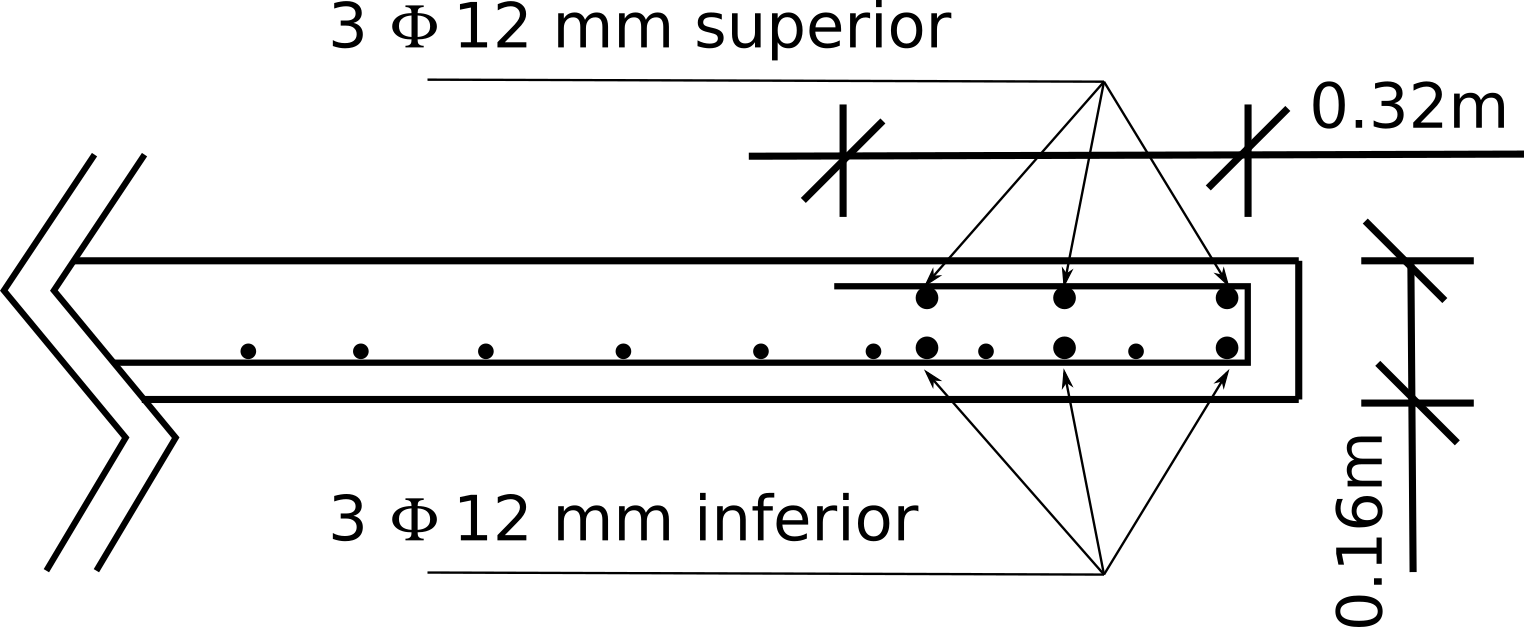
\includegraphics[scale = 1.2]{chapters/chapter_1/images/orificio2.png}
\end{center}
\end{figure}

\end{itemize}
\end{enumerate}